\documentclass[12pt, a4paper]{article}

\usepackage[utf8]{inputenc}
\usepackage{amsmath}
\usepackage{graphicx}
\usepackage{geometry}
\usepackage{xcolor}
\usepackage{listings}
\usepackage{float}

% Page geometry setup
\geometry{
    a4paper,
    left=25mm,
    right=25mm,
    top=25mm,
    bottom=25mm
}

% Code listing style setup
\definecolor{codegreen}{rgb}{0,0.6,0}
\definecolor{codegray}{rgb}{0.5,0.5,0.5}
\definecolor{codepurple}{rgb}{0.58,0,0.82}
\definecolor{backcolour}{rgb}{0.96,0.96,0.96}

\lstdefinestyle{pythonstyle}{
    backgroundcolor=\color{backcolour},   
    commentstyle=\color{codegreen},
    keywordstyle=\color{blue},
    numberstyle=\tiny\color{codegray},
    stringstyle=\color{codepurple},
    basicstyle=\ttfamily\footnotesize,
    breakatwhitespace=false,         
    breaklines=true,                 
    captionpos=b,                    
    keepspaces=true,                 
    numbers=left,                    
    numbersep=5pt,                  
    showspaces=false,                
    showstringspaces=false,
    showtabs=false,                  
    tabsize=4
}
\lstset{style=pythonstyle}

\title{Practical 5: MNIST and CNNs in PyTorch \\ \large Data Engineering 414}
\author{Jacob Johannes Mostert}
\date{\today}

\begin{document}

\maketitle

\section{Introduction}

This practical explores the implementation and evaluation of a Convolutional Neural Network (CNN) using the PyTorch framework. The primary objective is to build a model capable of accurately classifying handwritten digits from the MNIST dataset.

The core tasks require defining the convolutional and linear layers, and optimizing the network parameters through Stochastic Gradient Descent (SGD). By extracting and visualising the learned weights and activation maps, we aim to understand exactly how the network isolates distinct features to make its final classification decisions.

\section{The Data}

The initial phase of the practical required loading and verifying the MNIST dataset partitions. A predefined utility function extracted the feature vectors and corresponding target labels from compressed NumPy files. The dataset consists of images representing handwritten digits, which are flattened into 784-dimensional arrays.


\section{Convolutional Neural Network Architecture}

We built a Convolutional Neural Network (CNN) to extract visual features from the images and classify the digits. The network structure requires a 2D convolution layer, an activation function, and a final fully connected linear layer.

\subsection{Dimensionality and Math}
The first layer performs a 2D convolution. It takes an input image of height $P_1$ and width $P_2$ and slides a filter kernel of size $M_1 \times M_2$ across it. The amount the filter moves at each step is the stride ($S$). This operation produces an output feature map with new spatial dimensions, $Q_1$ and $Q_2$. We calculate these new dimensions using the following formulas:

\begin{equation}
    Q_1 = \left\lfloor \frac{P_1 - M_1}{S} \right\rfloor + 1
\end{equation}

\begin{equation}
    Q_2 = \left\lfloor \frac{P_2 - M_2}{S} \right\rfloor + 1
\end{equation}

Our input images are 28 pixels by 28 pixels ($P_1 = 28$, $P_2 = 28$). We set the kernel size to 8 by 8 ($M_1 = 8$, $M_2 = 8$) and the stride to $S = 2$. Plugging these values into the equations gives us an output size of 11 by 11. We configured the convolutional layer to output 10 channels ($M_3 = 10$). To pass this data into the final linear layer, we must flatten it into a single one-dimensional array. The total number of features entering the dense layer is therefore $11 \times 11 \times 10 = 1210$.

\subsection{Implementation}
In the model class, we set up the `nn.Conv2d` layer, the `nn.ReLU` activation, and the `nn.Linear` dense layer. The input data initially arrives as a flat array of 784 numbers. During the forward pass, we use the `view` function to reshape this array back into a 28 by 28 grid so the 2D convolution can process it correctly. After the convolution and activation steps, we flatten the tensor again before feeding it to the dense layer to get our final predictions.

\begin{lstlisting}[language=Python, caption=CNN Initialization and Forward Pass]
class CNN(nn.Module):
    def __init__(self, M_1, M_2, M_3, K, stride):
        super().__init__()
        
        self.conv_1 = nn.Conv2d(in_channels=1, out_channels=M_3, kernel_size=(M_1, M_2), stride=stride)
        self.relu_1 = nn.ReLU()

        Q1 = (28 - M_1) // stride + 1
        Q2 = (28 - M_2) // stride + 1
        dense_input_size = Q1 * Q2 * M_3

        self.dense = nn.Linear(in_features=dense_input_size, out_features=K)

    def forward(self, x):
        x_reshaped = x.view(-1, 1, 28, 28) 
        z_1 = self.conv_1(x_reshaped) 
        v_1 = self.relu_1(z_1) 
        v_1_flat = v_1.view(v_1.size(0), -1) 

        y_hat = self.dense(v_1_flat) 

        return y_hat, z_1, v_1
\end{lstlisting}

With the class defined, we created an instance of the model. We also set up the cross-entropy loss function and the Stochastic Gradient Descent (SGD) optimizer.

\begin{lstlisting}[language=Python, caption=Model Instantiation]
model = CNN(M_1=8, M_2=8, M_3=10, K=10, stride=2)
loss_fn = nn.CrossEntropyLoss()
optimizer = torch.optim.SGD(model.parameters(), lr=lr)
\end{lstlisting}


\section{Model Training and Optimization}

Training the model involves making predictions, calculating the error, and updating the network weights to reduce that error. We measure the error using the cross-entropy loss function, which compares the network's predictions against the actual correct labels.

We update the weights using the SGD optimizer. The mathematical update rule takes the current weights $\theta_t$, calculates the gradient of the loss $\nabla L(\theta_t)$, and scales it by a learning rate $\eta$ to find the new weights $\theta_{t+1}$:

\begin{equation}
    \theta_{t+1} = \theta_t - \eta \nabla L(\theta_t)
\end{equation}

In PyTorch, we must explicitly clear the old gradients before running a new backward pass. If we do not clear them using \texttt{optimizer.zero\_grad()}, the new gradients will add to the old ones and corrupt the training process. 

\begin{lstlisting}[language=Python]
# Training loop logic
optimizer.zero_grad() 
y_hat, z_1, v_1 = model(X_i) 
loss = loss_fn(y_hat, y_i) 
loss.backward() 
optimizer.step() 

# Test loop logic
y_hat, z_1, v_1 = model(X_i) 
loss = loss_fn(y_hat, y_i) 
\end{lstlisting}

We ran this training process for 10 epochs. The loss steadily decreased while the accuracy increased, showing that the model successfully learned to identify the digits.

\begin{figure}[H]
    \centering
    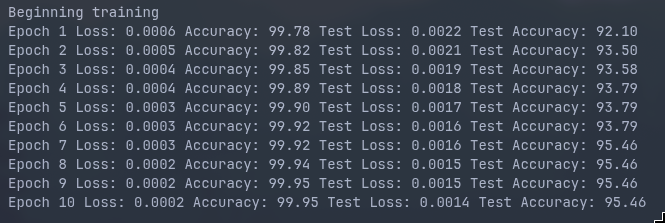
\includegraphics[width=0.8\textwidth]{images/3.png}
    \caption{Training progress showing decreasing loss and increasing accuracy.}
    \label{fig:output1}
\end{figure}


\section{Feature Map and Filter Visualisation}

To understand how the CNN processes images, we visualised the internal filters and output matrices for a single test image. We passed the first image from the test set through the model and extracted the weights from the convolutional layer.

The matrix $Z[1]$ represents the raw output directly after the convolution step. The matrix $V[1]$ shows the output after it passes through the ReLU activation function. The ReLU function works by converting all negative numbers to zero while leaving positive numbers unchanged. The formula is simply:

\begin{equation}
    V[1] = \max(0, Z[1])
\end{equation}

This thresholding operation adds non-linearity to the network. It allows the model to ignore unimportant features and focus only on the most prominent patterns.

\begin{lstlisting}[language=Python, caption=Extracting Weights and Visualising the First Example]
X = test_X[0,:] 
x_input = X[None,:] 

with torch.no_grad():
    y_hat, z_1, v_1 = model(x_input)

H = model.conv_1.weight

plot_filters(x_input, H, z_1, v_1) 
\end{lstlisting}

The plotted filters reveal that the network searches for specific shapes and edges. The final feature maps show how certain areas of the image strongly activate specific filters while the ReLU function completely suppresses the rest.

\begin{figure}[H]
    \centering
    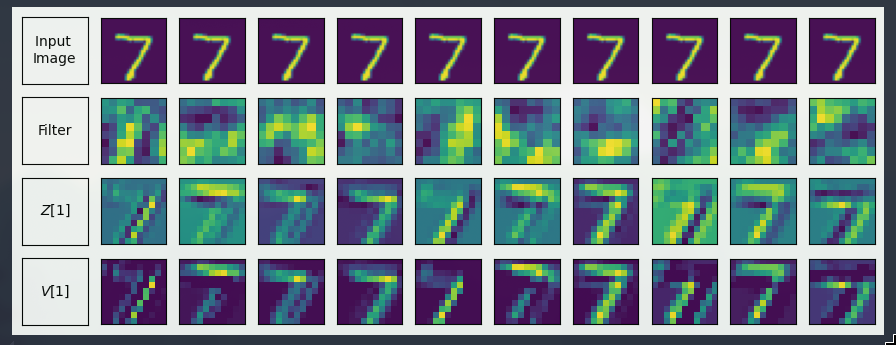
\includegraphics[width=0.8\textwidth]{images/1.png}
    \caption{Terminal output displaying the dimensions of the loaded training and testing tensors.}
    \label{fig:output3}
\end{figure}


\section{Class-Specific Activations}

To understand how the network differentiates between distinct shapes, we tested the model with three specific examples from our dataset. We selected indices 2, 3, and 5, representing the digits 1, 0, and 1. 

\subsection{Implementation Details}
The code iterates through our chosen indices using a standard loop. For each iteration, we extract the corresponding 784-dimensional image vector from the test set. 

A critical step before feeding this single image into the network is adjusting its shape. Because the CNN is designed to process batches of images simultaneously, it expects a four-dimensional input structure. We apply the \texttt{unsqueeze(0)} function to add a temporary batch dimension of size one. This ensures the geometric requirements of the convolution layer are met.

We then process the image inside a \texttt{torch.no\_grad()} block. During training, PyTorch actively tracks every mathematical operation to calculate gradients for the backward pass. Since we are strictly evaluating the model here, calculating gradients is unnecessary. Disabling this tracking reduces memory consumption and speeds up the forward pass. 

After the model generates its predictions (\texttt{y\_hat}), we use \texttt{torch.argmax} to identify the specific class with the highest probability score. Finally, we pass the extracted convolutional weights (\texttt{H}), the raw feature maps (\texttt{z\_1}), and the activated maps (\texttt{v\_1}) into the \texttt{plot\_filters} function to generate the visual grid.

\begin{lstlisting}[language=Python, caption=Testing Specific Digit Indices]
indices_to_test = [2, 3, 5] 

for idx in indices_to_test:
    X_experiment = test_X[idx,:]
    
    # Add a batch dimension for the CNN
    X_input = X_experiment.unsqueeze(0)
    
    # Disable gradient tracking for inference
    with torch.no_grad():
        y_hat, z_1, v_1 = model(X_input)
        
    H = model.conv_1.weight
    
    # Extract the highest probability prediction
    predicted_class = torch.argmax(y_hat, dim=-1).item()
    true_class = test_Y[idx].item()
    print(f"Index {idx} | True Class: {true_class} | Predicted Class: {predicted_class}")
    
    plot_filters(X_experiment, H, z_1, v_1)
    plt.show()
\end{lstlisting}

\subsection{Analysis of Filter Responses}
The visual output confirms our model predicted the correct class for all three inputs. More importantly, the feature maps reveal the underlying mechanics of convolutional feature extraction. 

Different digit morphologies trigger distinct responses across the ten filter channels. When the network processes the digit '1', filters optimized for straight vertical lines exhibit high activation values. Conversely, when the network evaluates the digit '0', those same vertical filters remain largely dormant. Instead, channels attuned to rounded edges and curved structures become highly active. This selective excitation creates a unique activation signature for every number. The final linear layer relies entirely on these distinct signatures to classify the images accurately.

\begin{figure}[H]
    \centering
    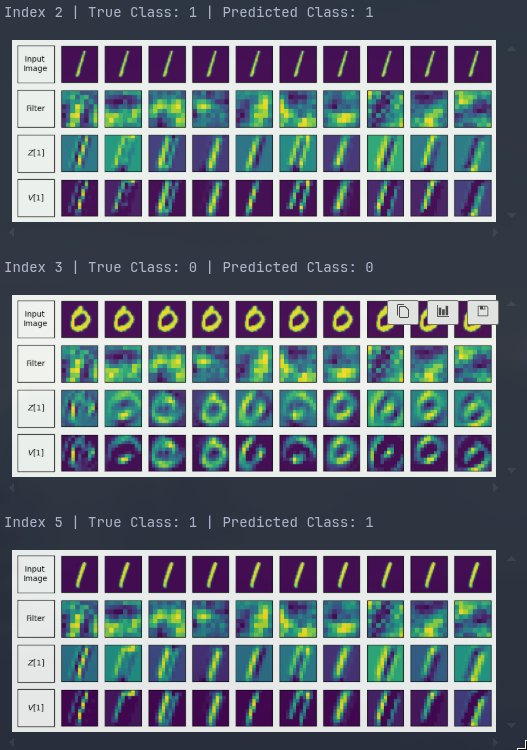
\includegraphics[width=0.8\textwidth]{images/2.png}
    \caption{Visualisation of the convolutional filters and feature maps for the selected test images.}
    \label{fig:output2}
\end{figure}

\section{Conclusion}
This practical provided a comprehensive exploration of Convolutional Neural Networks (CNNs) using the PyTorch framework. We successfully implemented a CNN architecture, trained it on the MNIST dataset, and visualised the learned filters and feature maps. The results demonstrated how the network extracts and processes visual features to classify handwritten digits accurately. By examining the activation patterns for specific digit examples, we gained insights into the internal workings of the CNN and how it differentiates between various classes based on learned features.

\end{document}